\documentclass[../../../../main.tex]{subfiles}

\begin{document}

\section*{第1問}

\begin{proof}[解]
$a>0$のもとで，$x\ge0,\ y\ge0,\ 2x+3y\le12,\ ax+\left(4-\dfrac{3a}2\right)y\le8$の表す領域を$D_a$とし，$D_a$上で$f=x+y$の最大値$f(a)$をもとめる。

\textbf{（鍵となる事実）} 直線$\ell_a:\ ax+\left(4-\dfrac{3a}2\right)y=8$は，$a$の値によらず定点$P(3,2)$を通る。実際
\[
3a+2\left(4-\frac{3a}2\right)=3a+8-3a=8
\]
であり，これは常に成立する。また$P(3,2)$は$2\cdot3+3\cdot2=12$より直線$2x+3y=12$上にもある。したがって2直線は常に$P(3,2)$で交わり，
\[
f(3,2)=5
\]

$f$は線形だから，$D_a$上の最大値は頂点でとる。$y=0$上では，$2x+3y\le12$から$x\le6$，$\ell_a$の制約$ax\le8$から$x\le8/a$であり，効くのは小さい方。$x=0$上では，$2x+3y\le12$から$y\le4$，$\ell_a$から$y\le16/(8-3a)$（$a<8/3$の時）であり，これも小さい方が効く。$16/(8-3a)$と$4$を比較すると$16-4(8-3a)=12a>0$（$a>0$）より常に$16/(8-3a)>4$なので，$x=0$上では常に$2x+3y\le12$の方が効き，$y$軸方向の頂点は常に$(0,4)$である（$f=4$，これが最大になることはない）。

\textbf{$1^\circ$ $0<a\le\dfrac43$の時}

$6a\le8$だから$x=6$（$y=0$上）は$\ell_a$の制約もみたし，$D_a$の頂点は$(6,0)$。$f(6,0)=6$であり，これは$(0,4)$の$4$，$P$の$5$より大きいので
\[
f(a)=6
\]

\textbf{$2^\circ$ $\dfrac43\le a\le\dfrac85$の時}

$6a\ge8$だから$x=6$は不適で，$y=0$上の頂点は$\ell_a$の$x$切片$\left(\dfrac8a,0\right)$になる。$a\le8/5\iff8/a\ge5$だから，この頂点での値$8/a$は$P$での値$5$以上であり，$(0,4)$の$4$より大きいので
\[
f(a)=\frac8a
\]

\textbf{$3^\circ$ $a\ge\dfrac85$の時}

$8/a\le5$となり，$y=0$上の頂点（存在する場合）での値は$P$の値$5$を超えない。実際，$a\ge8/3$では$4-\dfrac{3a}2\le0$となって$\ell_a$の$y$の係数の符号が反転し，制約$ax+(4-\tfrac{3a}2)y\le8$は$y\ge\dfrac{2ax-8}{3a-8}$の形（$y$の下限）に変わるが，このときも$D_a$の頂点は$(0,0),\left(\dfrac8a,0\right),P(3,2),(0,4)$のままで（$a=8/3$では$\ell_a$は垂直線$x=3$となり頂点は$(0,0),(3,0),P,(0,4)$），いずれの場合も最大値は$P$でとる。以上より
\[
f(a)=5
\]

以上をまとめて，
\[
f(a)=
\begin{cases}
6 & \left(0<a\le\dfrac43\right)\\[2mm]
\dfrac8a & \left(\dfrac43\le a\le\dfrac85\right)\\[2mm]
5 & \left(a\ge\dfrac85\right)
\end{cases}
\]

\begin{center}
\begin{tikzpicture}[scale=0.7, >=stealth]
  \draw[->] (-0.5,0) -- (7,0) node[right] {$x$};
  \draw[->] (0,-0.5) -- (0,5) node[above] {$y$};
  \draw[thick] (6,0) -- (0,4) node[above left] {$2x+3y=12$};
  \draw[thick,dashed] (4,0) -- (0,3.2) node[below left] {$\ell_a$（例）};
  \fill (3,2) circle (2pt) node[above right] {$P(3,2)$};
  \node[below] at (6,0) {$6$};
\end{tikzpicture}
\end{center}
\end{proof}

\newpage

\section*{第2問}

\begin{proof}[解]
長方形$R$の4頂点を，$X(0,a)$，$Y(b,a)$，$Z(b,0)$，$W(0,0)$とする（$XY=b$，$XW=a$，$0<a<b<2a$）。円$A$は性質(P)から2辺$XY,XW$に接するとしてよく，半径を$x$とすると中心は$(x,a-x)$であり，
\[
0<x<\frac a2 \quad\cdots\text{(＊)}
\]
が必要である。

\textbf{(1)} 円$A$に外接する性質(P)の円は，対称性から次の4つで尽くされる：頂点$W$で2辺$XW,WZ$に接する円$C_1$（半径$r_1$，中心$(r_1,r_1)$），頂点$Z$で2辺$WZ,ZY$に接する円$C_2$（半径$r_2$，中心$(b-r_2,r_2)$），頂点$Y$で2辺$ZY,YX$に接する円$C_3$（半径$r_3$，中心$(b-r_3,a-r_3)$），そして頂点$X$で円$A$と同じ2辺$XY,XW$に接し，$A$より角$X$寄りにある円$C_4$（半径$r_4$，中心$(r_4,a-r_4)$）。

\textbf{$C_1$について：} $A,C_1$が外接する条件から
\[
(x-r_1)^2+(a-x-r_1)^2=(x+r_1)^2
\]
整理すると（$a-x-r_1>0$に注意して）
\[
(a-x-r_1)^2=4xr_1 \quad\therefore\ a-x-r_1=2\sqrt{xr_1}
\]
\[
a=x+r_1+2\sqrt{xr_1}=(\sqrt x+\sqrt{r_1})^2 \quad\therefore\ r_1=(\sqrt a-\sqrt x)^2
\]

\textbf{$C_3$について：} 同様に
\[
(b-x-r_3)^2+(x-r_3)^2=(x+r_3)^2 \ \Longrightarrow\ b=x+r_3+2\sqrt{xr_3}=(\sqrt x+\sqrt{r_3})^2
\]
\[
\therefore\ r_3=(\sqrt b-\sqrt x)^2
\]

\textbf{$C_2$について：} $A,C_2$が外接する条件から
\[
(b-x-r_2)^2+(a-x-r_2)^2=(x+r_2)^2
\]
展開して整理すると
\[
(x+r_2)^2-2(a+b)(x+r_2)+a^2+b^2=0
\]
$u=x+r_2$とおくと$u^2-2(a+b)u+(a^2+b^2)=0$より
\[
u=(a+b)\pm\sqrt{2ab}
\]
複号のうち$+$は$r_2$が大きくなりすぎ図形的制約に反するので不適，
\[
r_2=(a+b)-\sqrt{2ab}-x
\]

\textbf{$C_4$について：} $A,C_4$は同じ角$X$の二等分線上に中心があり，外接条件から中心間距離$\sqrt2(x-r_4)=x+r_4$（$r_4<x$）。よって
\[
\sqrt2\,x-\sqrt2\,r_4=x+r_4 \quad\therefore\ r_4=\frac{(\sqrt2-1)x}{\sqrt2+1}=(3-2\sqrt2)x
\]

$r_1=(\sqrt a-\sqrt x)^2$が意味を持ち，かつ$0<r_1<a/2$をみたすことなどから，$0<r_k<a/2$（$k=1,2,3$）の存在条件を調べればよい。$r_1<a/2$の条件は$\sqrt a-\sqrt x<\sqrt{a/2}$，$r_3<a/2$の条件は$\sqrt b-\sqrt x<\sqrt{a/2}$であり，$b>a$からこちらがより強い条件を与える：
\[
\sqrt x>\sqrt b-\sqrt{\frac a2} \quad\therefore\ x>\left(\sqrt b-\sqrt{\frac a2}\right)^2
\]
（$r_2$を与える$u$の方程式は判別式$(a+b)^2-(a^2+b^2)=2ab>0$から常に解をもち，$r_2$は自動的に存在する。）以上と(＊)をあわせて，もとめる条件は
\[
\left(\sqrt b-\sqrt{\frac a2}\right)^2<x<\frac a2
\]

\begin{center}
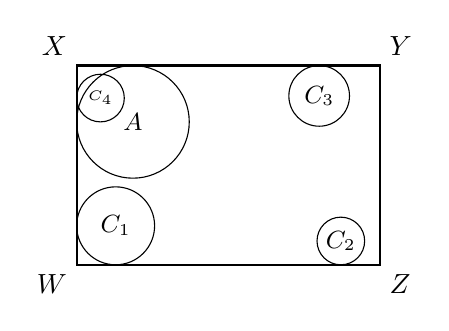
\begin{tikzpicture}[scale=0.55, >=stealth]
  \draw[thick] (0,0) rectangle (7,4.6);
  \node[below left] at (0,0) {$W$};
  \node[below right] at (7,0) {$Z$};
  \node[above right] at (7,4.6) {$Y$};
  \node[above left] at (0,4.6) {$X$};
  \draw (1.3,3.3) circle (1.3);
  \draw (0.55,3.85) circle (0.55);
  \draw (0.9,0.9) circle (0.9);
  \draw (6.1,0.55) circle (0.55);
  \draw (5.6,3.9) circle (0.7);
  \node at (1.3,3.3) {\small$A$};
  \node at (0.9,0.9) {\small$C_1$};
  \node at (6.1,0.55) {\small$C_2$};
  \node at (5.6,3.9) {\small$C_3$};
  \node at (0.55,3.85) {\tiny$C_4$};
\end{tikzpicture}
\end{center}

\textbf{(2)} (1)の条件下で，まず$C_4$の半径$r_4=(3-2\sqrt2)x$は$3-2\sqrt2\approx0.17$と小さいため，常に$r_1$より小さい（実際$r_1=(\sqrt a-\sqrt x)^2$は$x<a/2$の範囲で$r_4$より大きいことが確かめられる）。また
\[
r_3-r_2=(b+x-2\sqrt{bx})-\bigl((a+b)-\sqrt{2ab}-x\bigr)=2x-2\sqrt{bx}+\sqrt{2ab}-a
\]
\[
=2\left(\sqrt x-\frac{\sqrt{2a}}2\right)\left(\sqrt x-\frac{2\sqrt b-\sqrt{2a}}2\right)
\]
(1)の範囲内でこれが負であることが確かめられるので，$r_3<r_2$。以上から4円の半径の大小は
\[
r_2>r_3>r_1>r_4
\]
となり，$A$に外接する4円のうち「2番目に大きい円」$B$は半径$r_3$の$C_3$である。

したがって$A$と$B$の面積の和$S$は
\[
S=\pi\left(x^2+r_3^2\right)=\pi\left\{x^2+(\sqrt b-\sqrt x)^4\right\}
\]
$X=\sqrt x$とおいて微分すると
\[
\frac{dS}{dx}=\pi\left\{2x+4(\sqrt x-\sqrt b)^3\cdot\frac1{2\sqrt x}\right\}=\pi\left\{2X^2+\frac{2(X-\sqrt b)^3}{X}\right\}
\]
\[
=\frac{2\pi}{X}\left\{X^3+X^3-3\sqrt bX^2+3bX-b\sqrt b\right\}=\frac{4\pi}{X}\left(X-\frac{\sqrt b}2\right)\left(X^2-\sqrt bX+b\right)
\]
\[
=\frac{4\pi}{X}\left(X-\frac{\sqrt b}2\right)\left\{\left(X-\frac{\sqrt b}2\right)^2+\frac{3b}4\right\}
\]
$\{\ \cdots\ \}$の中は常に正だから，$dS/dx$の符号は$X-\sqrt b/2$の符号と一致し，(1)の範囲$\sqrt b-\sqrt{a/2}<X<\sqrt{a/2}$の中に$X=\sqrt b/2$が含まれる（$2a>b$より$\sqrt b/2<\sqrt{a/2}$）ので，下表を得る。
\begin{center}
\begin{tabular}{c|ccccc}
$X$ & $\sqrt b-\sqrt{a/2}$ & & $\sqrt b/2$ & & $\sqrt{a/2}$ \\
\hline
$S'$ & & $-$ & $0$ & $+$ & \\
\hline
$S$ & & $\searrow$ & & $\nearrow$ &
\end{tabular}
\end{center}
よって$X=\sqrt b/2$，すなわち$x=b/4$で$S$は最小となり，この時$r_3=(\sqrt b-\sqrt{b/4})^2=(\sqrt b/2)^2=b/4$だから
\[
\min S=\pi\left\{\left(\frac b4\right)^2+\left(\frac b4\right)^2\right\}=\frac{b^2}{8}\pi
\]
\end{proof}

\newpage

\section*{第3問}

\begin{proof}[解]
$f(x)=\dfrac{2x-1}x$，$f_0(t)=t$，$f_n(t)=f(f_{n-1}(t))$とする。

\textbf{(1)} $f_{n+1}(t)$が定義できるためには$f_n(t)\ne0$が必要（分母）。そこで各$n\ge0$に対し$f_n(t)=0$となる$t$を帰納的にもとめる。

$f_0(t)=0\iff t=0=\dfrac0{0+1}$。$n=k$で「$f_k(t)=0\iff t=\dfrac k{k+1}$」が成り立つと仮定する。$f_{k+1}(t)=0$の時，$f_k(t)=t'$とおくと$f_{k+1}(t)=f(t')=\dfrac{2t'-1}{t'}=0\iff t'=\dfrac12$。すなわち$f_k(t)=\dfrac12$。仮定の漸化式の構造から（$f_k$の定義式を用いて逆算すると）これをみたす$t$は
\[
t=\frac{k+1}{k+2}
\]
となる。以上により$n\in\mathbb N$のすべてに対し
\[
f_n(t)=0\iff t=\frac n{n+1}
\]
が成り立つ。したがって，すべての$n$に対し$f_n(t)$が矛盾なく（分母が$0$にならず）定義できるための$t$の条件は
\[
t\ne\frac n{n+1}\quad(n\in\mathbb N)
\]

\textbf{(2)} $g_n(t)=f_n(t)-1$とおく。$f_{n+1}=2-\dfrac1{f_n}$だから
\[
g_{n+1}(t)=f_{n+1}(t)-1=1-\frac1{f_n(t)}=\frac{f_n(t)-1}{f_n(t)}=\frac{g_n(t)}{g_n(t)+1}\quad\cdots\text{①}
\]
$g_0(t)=t-1$である。$g_k(t)=\dfrac{t-1}{k(t-1)+1}$と予想して帰納法で示す。$k=0$で成立。①に代入すると
\[
g_{k+1}(t)=\frac{\dfrac{t-1}{k(t-1)+1}}{\dfrac{t-1}{k(t-1)+1}+1}=\frac{t-1}{(t-1)+k(t-1)+1}=\frac{t-1}{(k+1)(t-1)+1}
\]
となり，$k+1$でも成立。よって
\[
g_n(t)=\frac{t-1}{n(t-1)+1}=\frac1n-\frac1{n^2(t-1)+n}
\]

$a\ge1$として，
\[
n^2\int_a^{a+\frac1n}g_n(t)\,dt=n^2\left[\frac tn-\frac1{n^2}\log\bigl(n(t-1)+1\bigr)\right]_a^{a+\frac1n}
\]
\[
=n^2\left[\frac1{n^2}-\frac1{n^2}\log\frac{n(a-1)+2}{n(a-1)+1}\right]=1-\log\left(a-1+\frac2n\right)+\log\left(a-1+\frac1n\right)
\]

$a>1$の時，$n\to\infty$で$\log(a-1+2/n)\to\log(a-1)$，$\log(a-1+1/n)\to\log(a-1)$となるので
\[
n^2\int_a^{a+\frac1n}(f_n(t)-1)\,dt\longrightarrow1
\]
$a=1$の時は
\[
1-\log\frac2n+\log\frac1n=1+\log\frac{1/n}{2/n}=1+\log\frac12=1-\log2
\]
（$n$によらず一定）。以上をまとめて，もとめる極限値は
\[
\lim_{n\to\infty}n^2\int_a^{a+\frac1n}(f_n(t)-1)\,dt=
\begin{cases}
1-\log2 & (a=1)\\
1 & (a>1)
\end{cases}
\]
\end{proof}

\newpage

\section*{第4問}

\begin{proof}[解]
楕円$C:\dfrac{x^2}{a^2}+y^2=1$（$a>1$），$A(a,0)$，$B(a\cos\theta,\sin\theta)$（$0<\theta<\pi$，$q=\sin\theta>0$）とし，$c=\cos\theta,\ s=\sin\theta$と書く。$B$における接線は
\[
\ell:\ \frac{p}{a^2}x+qy=1,\qquad p=ac,\ q=s
\]

$\ell$の方向ベクトルは$\vec\ell=(-as,c)$，直線$x=p$の方向ベクトルは$(0,1)$，$\overrightarrow{BA}=(a(1-c),-s)$である。2直線のなす角の正接は，方向ベクトル$\vec u,\vec v$に対し$\tan=\dfrac{|\vec u\times\vec v|}{\vec u\cdot\vec v}$（外積は$z$成分）で計算できるから，

$\ell$と$x=p$のなす角$\beta$について，角は鋭角にとるので絶対値を用いて
\[
\vec\ell\times(0,1)=-as,\qquad \vec\ell\cdot(0,1)=c \quad\therefore\ \tan\beta=\frac{as}{|c|}
\]

$\ell$と$BA$のなす角$\alpha$について，
\[
\vec\ell\times\overrightarrow{BA}=(-as)(-s)-c\cdot a(1-c)=a(s^2-c+c^2)=a(1-c)
\]
\[
\vec\ell\cdot\overrightarrow{BA}=-a^2s(1-c)-cs=-s\{a^2(1-c)+c\}
\]
$a^2(1-c)+c>0$（$1-c>0$かつ$a>1$から常に成立）なので
\[
\therefore\ \tan\alpha=\frac{a(1-c)}{s\{a^2(1-c)+c\}}
\]

条件$\alpha=\beta$（ともに鋭角）より$\tan\alpha=\tan\beta$：
\[
\frac{a(1-c)}{s\{a^2(1-c)+c\}}=\frac{as}{|c|}
\]
\[
|c|(1-c)=s^2\{a^2(1-c)+c\}=(1-c)(1+c)\{a^2(1-c)+c\}
\]
$1-c\ne0$（$B\ne A$）で両辺を割って
\[
|c|=(1+c)\{a^2(1-c)+c\}
\]
まず$c>0$（$|c|=c$）と仮定すると，$c=(1+c)\{a^2(1-c)+c\}$を整理して$a^2+(1-a^2)c^2=0\ \therefore\ c^2=\dfrac{a^2}{a^2-1}>1$となり$0<c<1$に反し不適。よって$c<0$（$|c|=-c$）であり，
\[
-c=(1+c)\{a^2(1-c)+c\}
\]
\[
0=c+(1+c)\{a^2(1-c)+c\}
\]
右辺を展開すると（$a^2(1-c)+c=a^2-a^2c+c$に注意して）
\[
(1+c)\{a^2(1-c)+c\}=(a^2-a^2c+c)+c(a^2-a^2c+c)=a^2+c+(1-a^2)c^2
\]
だから
\[
0=c+a^2+c+(1-a^2)c^2=(1-a^2)c^2+2c+a^2 \quad\therefore\ (a^2-1)c^2-2c-a^2=0
\]
\[
c=\frac{1\pm\sqrt{1+a^2(a^2-1)}}{a^2-1}
\]
$c<0$かつ$a>1$（$a^2-1>0$）より，$+$の解は常に正だから不適。よって
\[
c=\frac{1-\sqrt{1+a^2(a^2-1)}}{a^2-1}
\]
（これは確かに負：$\sqrt{1+a^2(a^2-1)}>1$だから分子は負。）

\textbf{(1)} 求める$p$は
\[
p=ac=\frac{a\left\{1-\sqrt{1+a^2(a^2-1)}\right\}}{a^2-1}
\]

\textbf{(2)} 分子を有理化すると
\[
p=\frac{a\left\{1-\bigl(1+a^2(a^2-1)\bigr)\right\}}{(a^2-1)\left\{1+\sqrt{1+a^2(a^2-1)}\right\}}=\frac{-a^3(a^2-1)}{(a^2-1)\left\{1+\sqrt{1+a^2(a^2-1)}\right\}}=\frac{-a^3}{1+\sqrt{1+a^2(a^2-1)}}
\]
したがって
\[
\lim_{a\to1}p=\frac{-1}{1+\sqrt1}=-\frac12
\]

また，
\[
\frac pa=\frac{1-\sqrt{1+a^2(a^2-1)}}{a^2-1}=\frac{\dfrac1{a^2}-\sqrt{\dfrac1{a^4}+1-\dfrac1{a^2}}}{1-\dfrac1{a^2}}
\]
$a\to\infty$の時，$1/a^2\to0,\ 1/a^4\to0$だから
\[
\lim_{a\to\infty}\frac pa=\frac{0-\sqrt1}{1-0}=-1
\]
\end{proof}

\end{document}
